\clearpage
\section{The new model}
\label{sec:model}
The FjordOs CL model is based on version 3.6 of the Rutgers Regional Ocean Modeling System (ROMS) adapted to the Oslofjord. ROMS is an open source, numerical ocean model as detailed and documented by \cite{haidv:etal:2008}, \cite{shche:mcwil:2003} and \cite{shche:mcwil:2005, shche:mcwil:2009}. It is freely available and may be downloaded from the ROMS website\footnote{\texttt{http://www.myroms.org/}}. 

In summary ROMS is a free-surface and terrain-following, vertical coordinate ocean model, based on the fully three-dimensional, rotational RANS\footnote{Reynolds Average Navier-Stokes} equations utilizing the hydrostatic and Boussinesq approximations. It is a so called split–explicit model where short time steps are used to advance the surface elevation and barotropic momentum equation, and where a much larger time step is used for temperature, salinity, and baroclinic momentum. In this ROMS employs a two-way time-averaging procedure for the barotropic mode which satisfies the 3D continuity equation. 

% % % % % % % % % % % % % % % % % % % % % % % % % % % % % % % % 
\subsection{Why ROMS?}
An option in ROMS is to use a curvilinear, near orthogonal grid to replace the default orthogonal regular mesh. This option is exploited here. The rationale is that it allows us to minimize the number of, or in reality the area of, ``dry'' grid points. Thereby the number of ``wet'' grid points is maximized without increasing the number of grid points compared to an orthogonal, regular grid mesh model covering the same domain. Thus resolution is increased without increasing the computational burden. In addition it allows us, to a certain extent, to put higher resolution in areas of special interest.
%%%%%%%%%%%%%%%%%%%%%%%%%%%% Figure 6 General curvilinear model %%%%%%%%%%%%%%%%%%%%
\begin{figure}[t]
 \begin{center}
  \begin{pspicture}(0,0)(15,11)
% Include graphs
   \rput[b](7.5,0.0){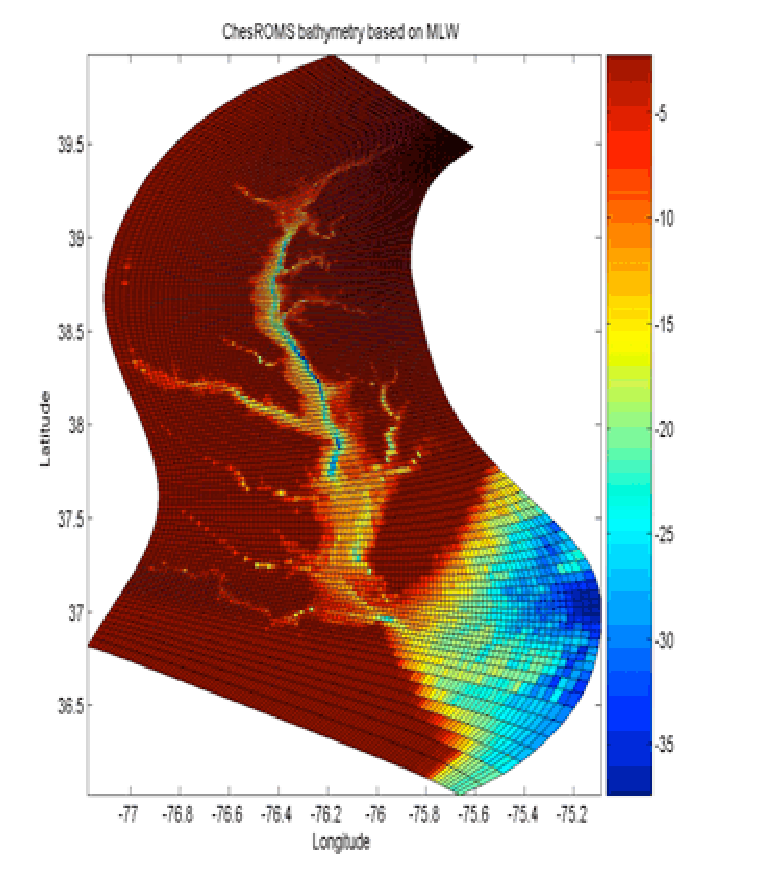
\includegraphics[height=11cm]{ChesROMS_grid}}
  \end{pspicture}
  \caption{\small Examples of a curvilinear grid showing the curvlinear grid used for the Cheasapeake Bay model ChesROMS. Note how the grids follows the land/sea matrix, thus minimizing the number of ``dry'' points. Likewise note how the grid size varies in space.} 
  \label{fig:curvil}
 \end{center}
\end{figure}



The above may also be achieved using unstructured grid models (e.g., FVCOM\footnote{\texttt{http://fvcom.smast.umassd.edu/fvcom/}}, SLIM\footnote{\texttt{http://sites.uclouvain.be/slim/}}). However, the FjordOs research group opted to go for a ROMS development utilizing its curvilinear option rather than starting a completely new strand of model development. The rationale is that 1) ROMS is MET Norway's operational model, 2) MET Norway's scientists are well versed in using ROMS, and 3) MET Norway's scientists have the necessary expertise to operate it. Moreover, none of researchers within the FjordOs participating institutions have any beforehand experience in running and/or setting up a three-dimensional, unstructured model. Nevertheless, to get some insight into the capabilities of an unstructured model, a \emph{two-dimensional version} of FVCOM was used as part of the FjordOs project for the work regarding Moss Harbor \citep{hjelm:etal:2014}.  
%%%%%%%%%%%%%%%%%%%%%%%%%%% Figure 9 FjordOs sketch %%%%%%%%%%%%%%%%%%%%
\begin{figure}[t]
 \begin{center}
  \begin{pspicture}(0,0)(15,10)
   \rput[bl]( 0.0,0.0){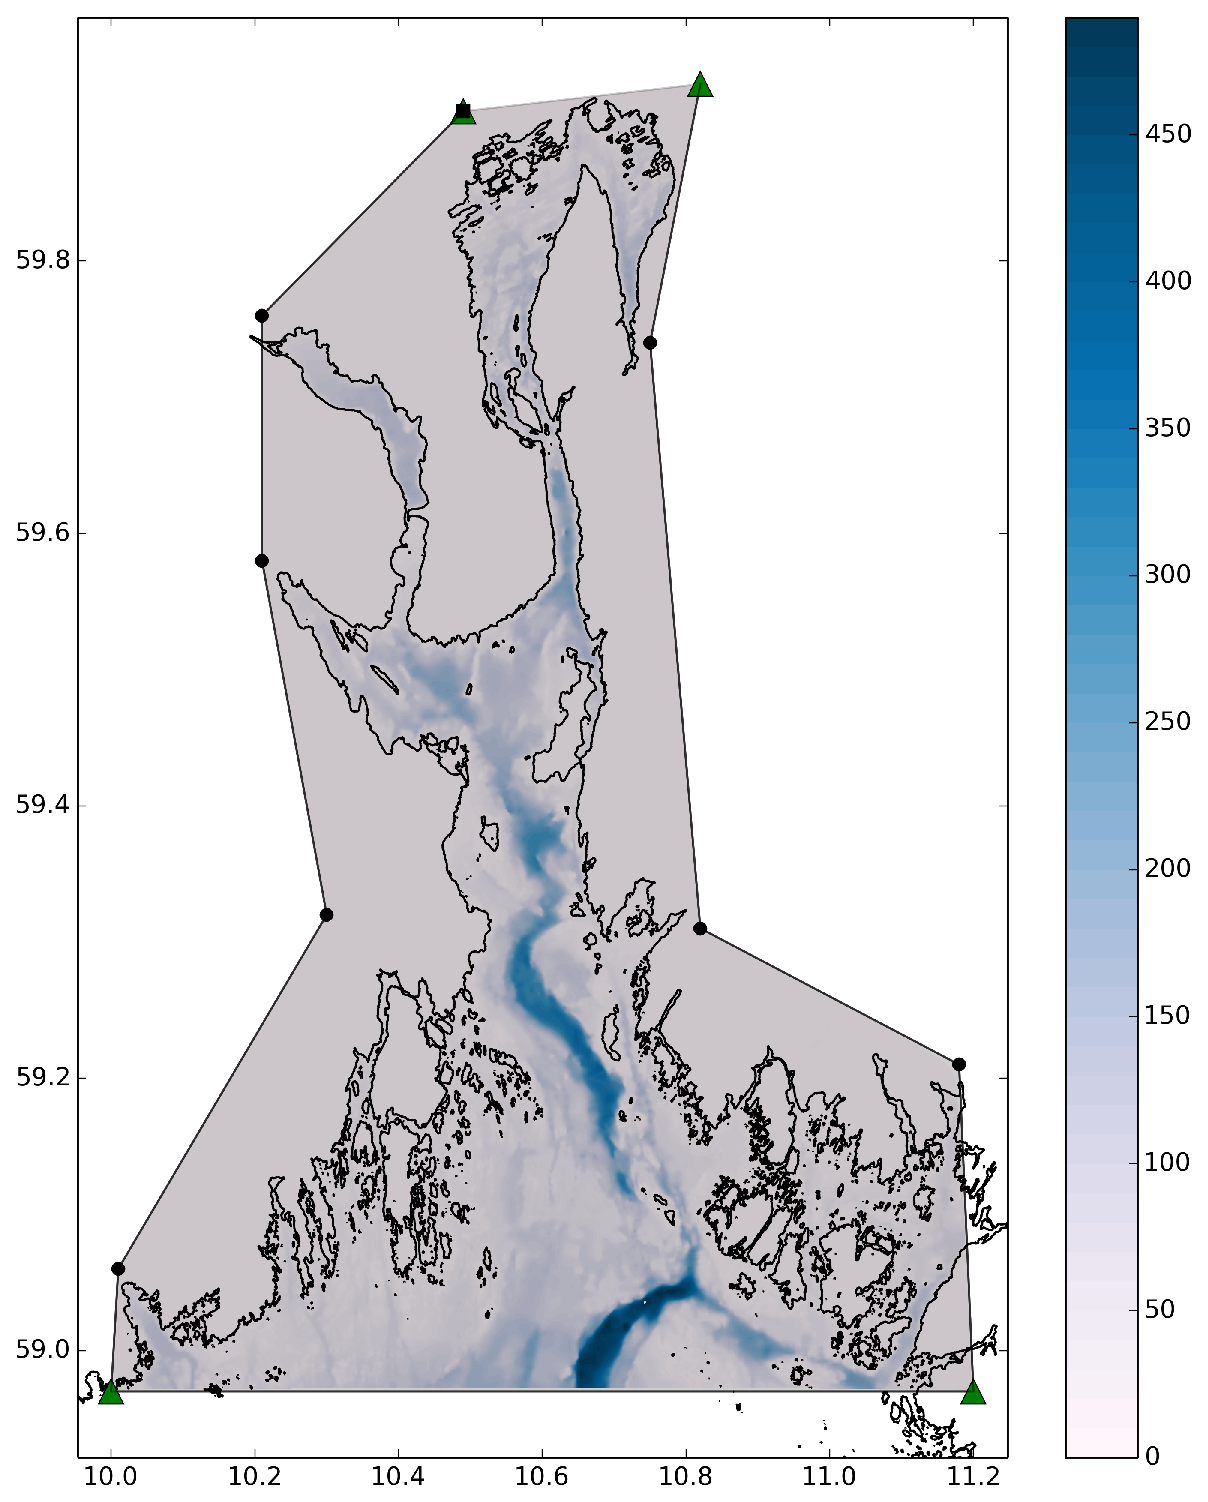
\includegraphics[height=9.0cm]{fig4_crop}}
   \rput[br](15.0,0.0){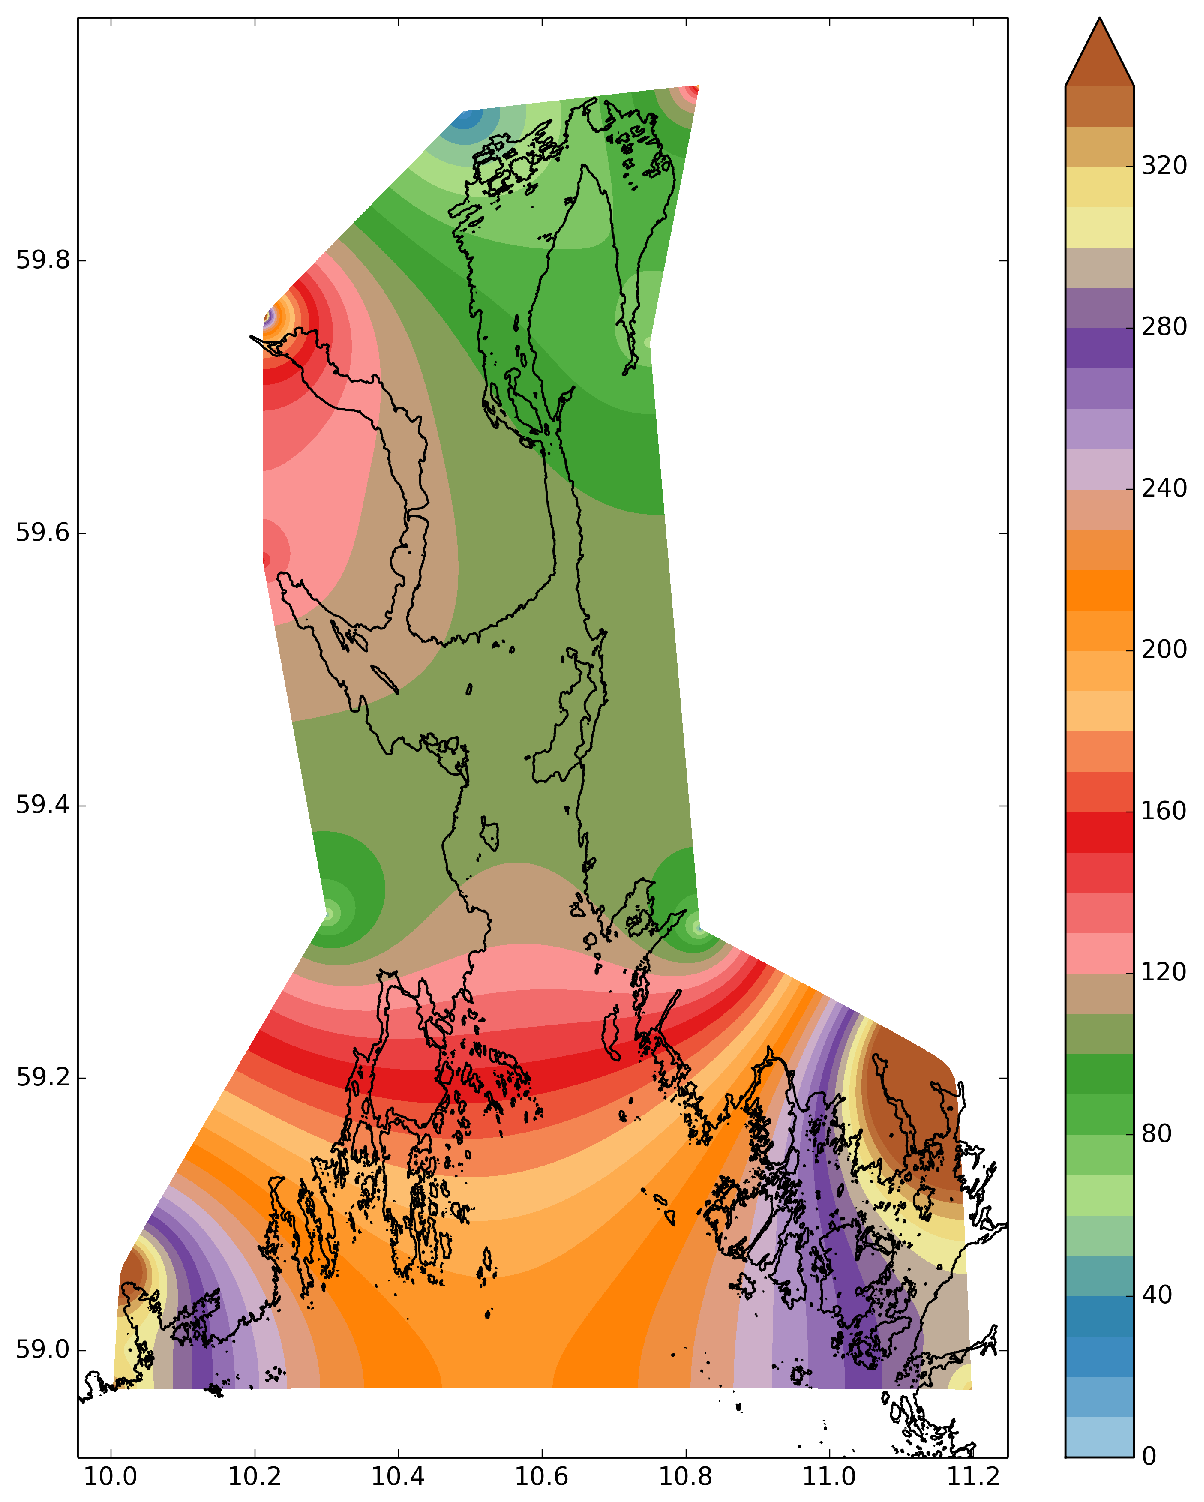
\includegraphics[height=9.0cm]{res_crop}}
   \rput[bl]( 5.0,5.0){\textbf{a)}}
   \rput[br](13.0,5.0){\textbf{b)}}
  \end{pspicture}
  \caption{\small The FjordOs CL computational domain showing (a) the curvilinear grid configuration, and (b) the resulting grid resolution. The right-hand color bar indicates grid size in meters, while the left-hand bluescaled colorbar indicates depth in meters. X-axis is degrees east, and y-axis is degrees north.} 
  \label{fig:fjordos_grid}
 \end{center}
\end{figure}

   

% % % % % % % % % % % % % % % % % % % % % % % % % % % % % % % % 
\subsection{The curvilinear FjordOs CL grid}
Our implementation is inspired in parts by models like the ChesROMS\footnote{\texttt{http://ches.communitymodeling.org/models/ChesROMS/}} model that applied the curvilinear option for an implementation of ROMS for Chesapeake Bay. There exists several different software packages (MATLAB, Fortran, Python, etc.) that can be used for creating curvilinear grids with variable horizontal resolution for ROMS. We use the python-based software package OCTANT\footnote{\texttt{https://github.com/hetland/octant}}. The outer borders of the model domain is defined by corners and nodes as depicted in Figure \ref{fig:fjordos_grid} where corners are depicted as triangles and the nodes as circular dots. There should be a total of exactly four corners to limit the domain. ``Bends'' or nodes in the side walls are then specified so as to follow the land-sea matrix. For this first version of the FjordOs model, we have chosen the corners and nodes using a ``trial-and-error'' approach, so the geometry might be changed in future versions of the FjordOs CL model.
%%%%%%%%%%%%%%%%%%%%%%%%%%% Figure 8 FjordOs ROMS %%%%%%%%%%%%%%%%%%%%
\begin{figure}[t]
 \begin{center}
  \begin{pspicture}(0,0)(15,11)
%  \begin{pspicture}(0,0)(15,18.5)
% Include graphs (the ratio of height to width must be 18.5/8)
% Stående
   \rput[b](7.5,0.0){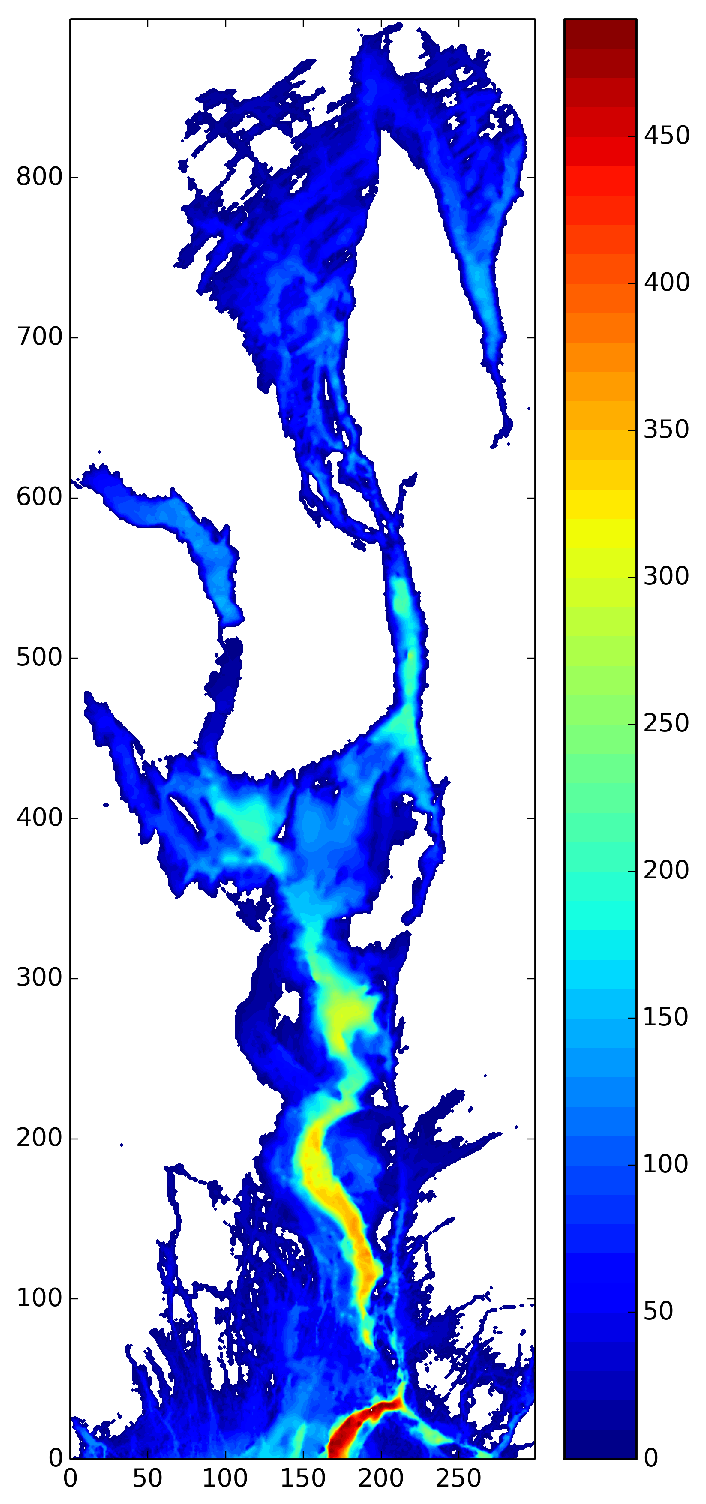
\includegraphics[height=11cm]{fjordos_cl}}
% Liggende
%   \rput[b]( 7.5,0.0){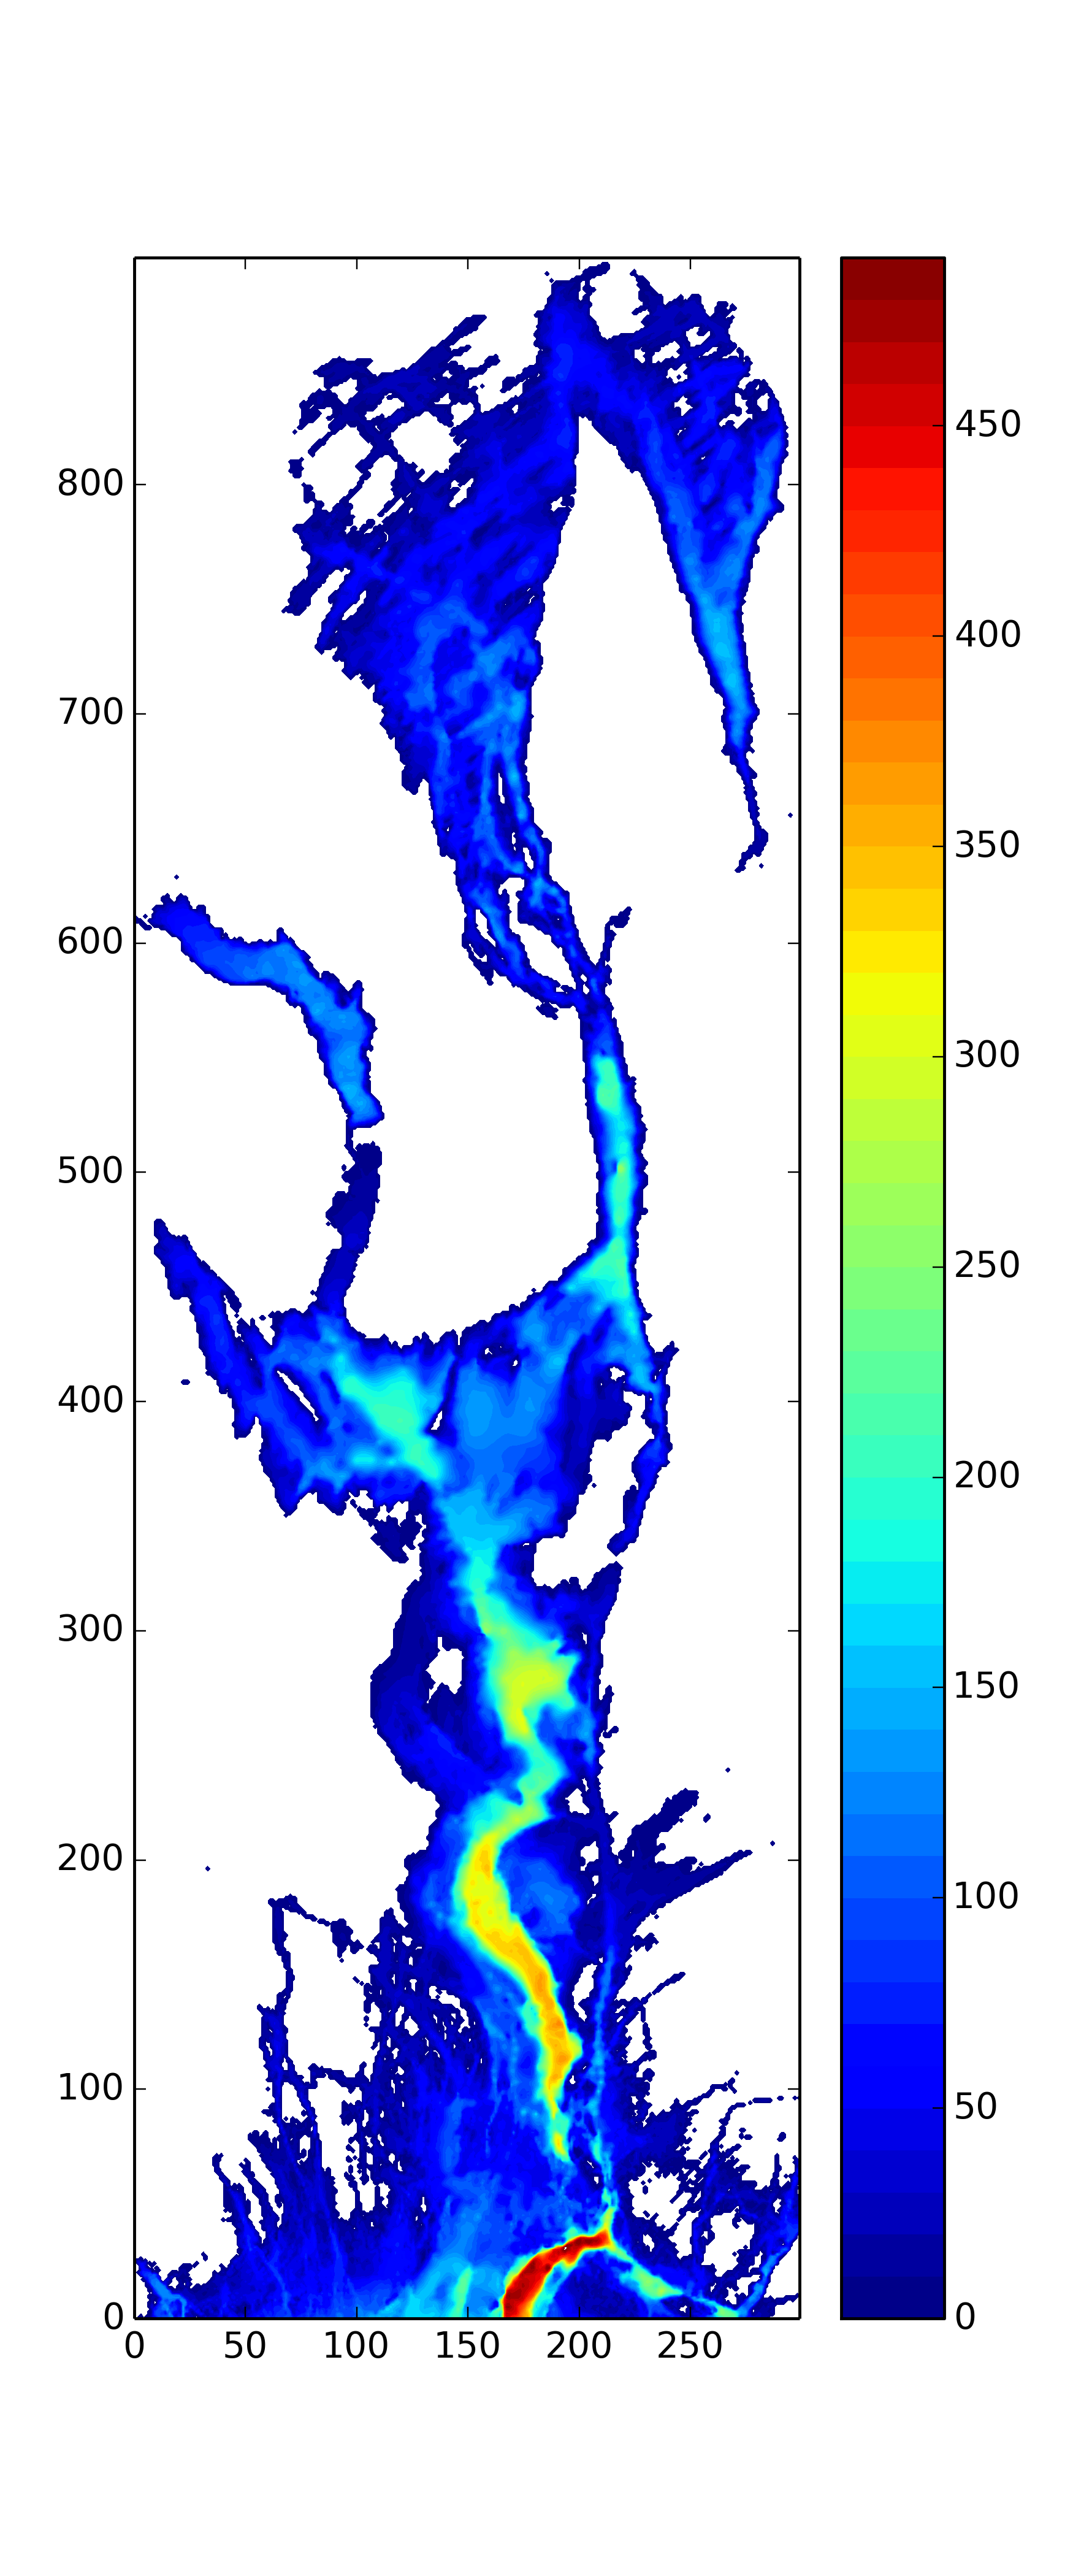
\includegraphics[angle=90,width=15.0cm,height=6.4865cm]{fjordos_roms}}
%   \rput[b]( 7.5,0.0){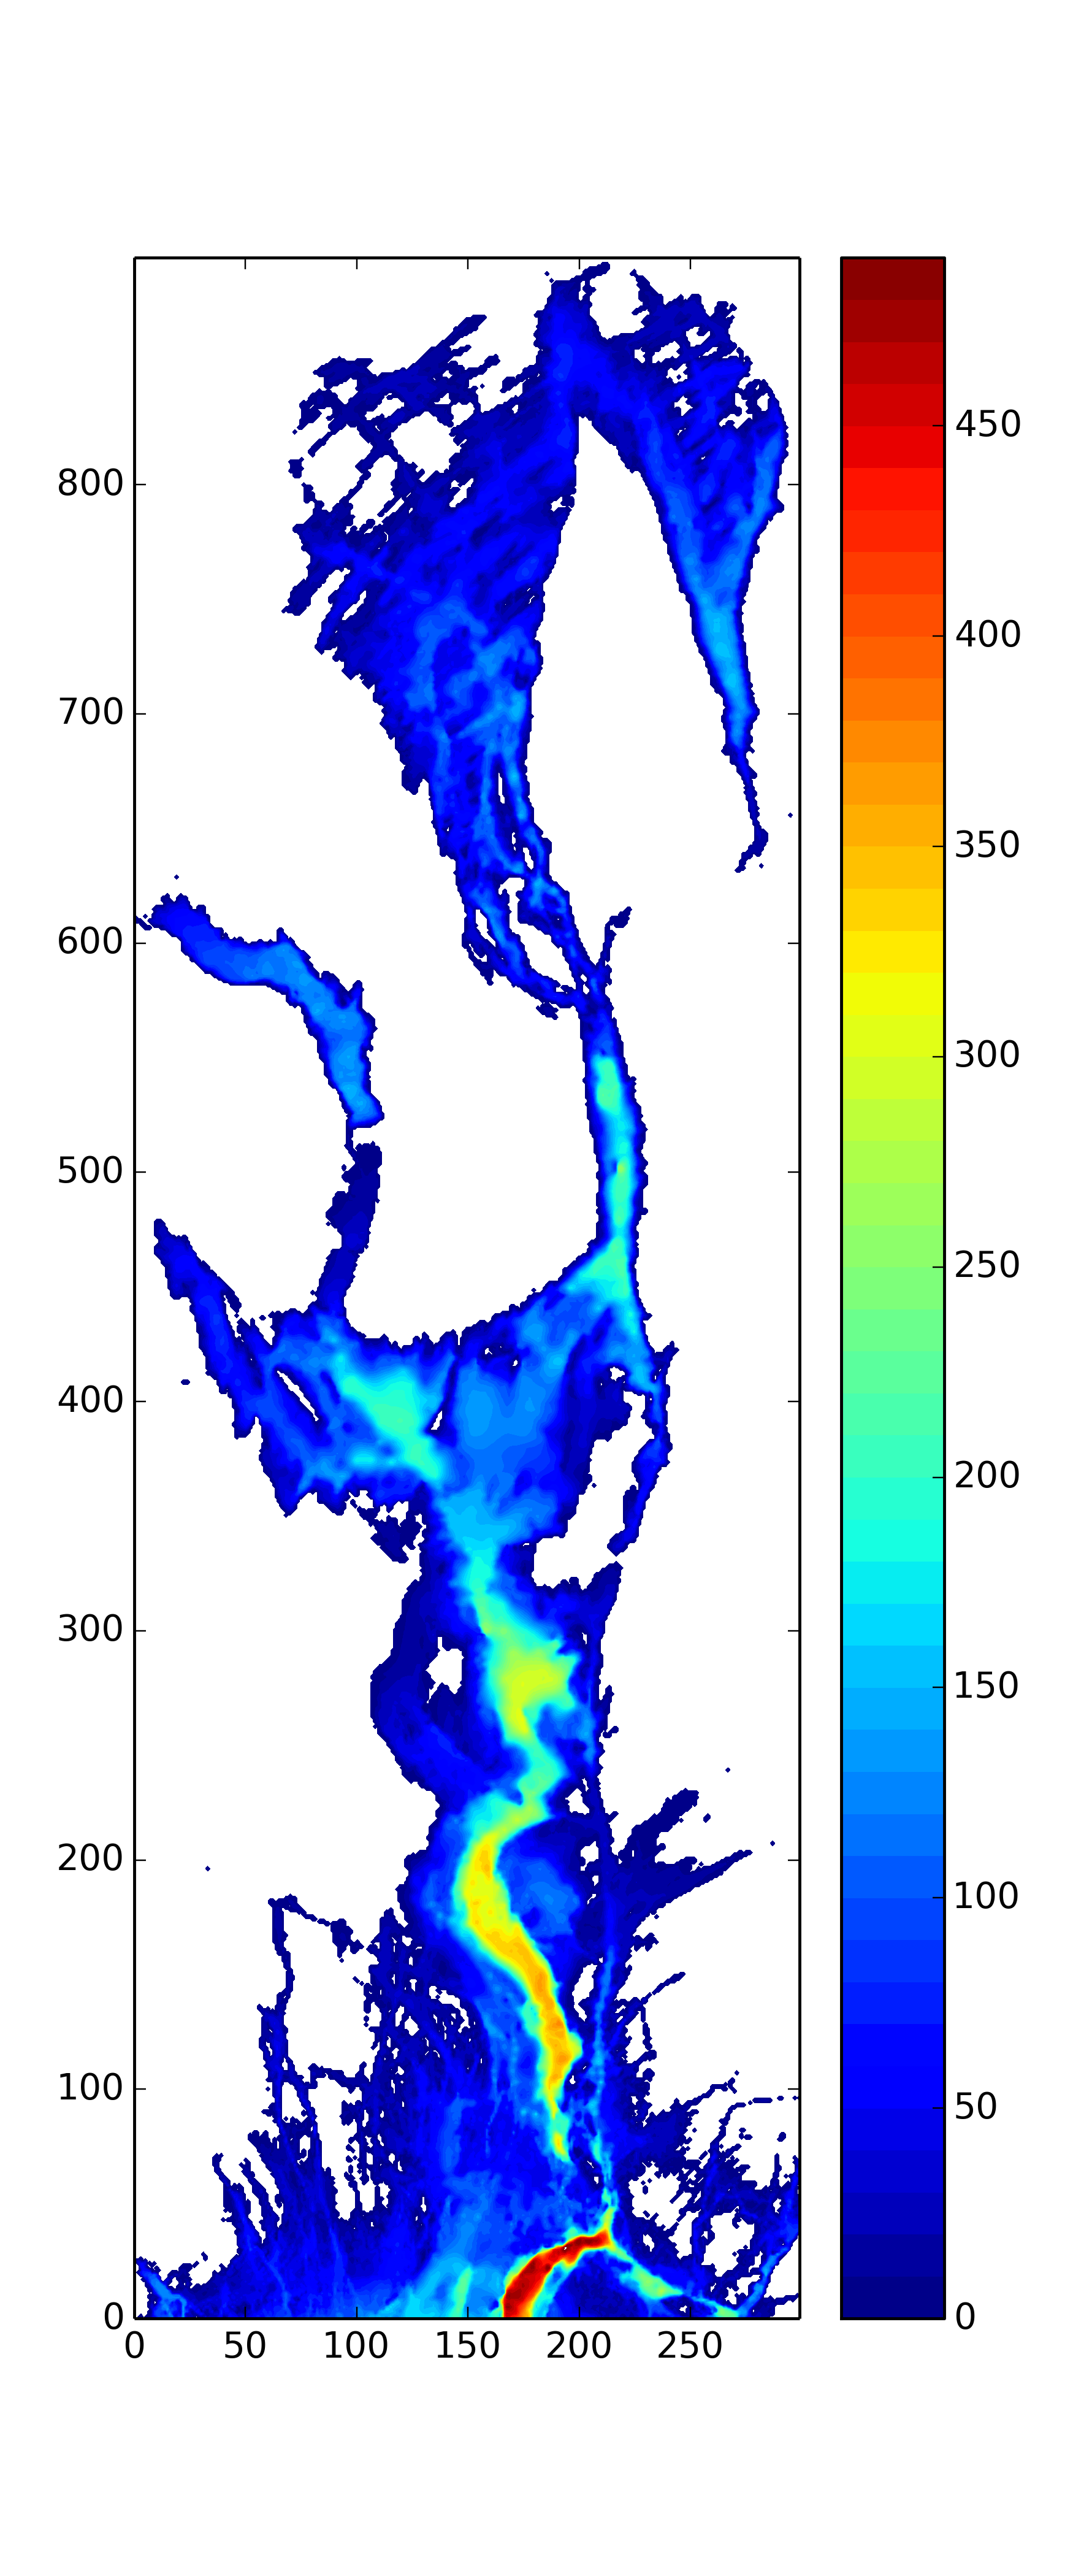
\includegraphics[height=8cm]{fjordos_roms}}
  \end{pspicture}
  \caption{\small The transformed curvilinear grid of the Oslofjord. The colors gives the depth in meters according to the color bar to the right. Model grid numbers associated with the curvilinear grid are given along the axes. There are 300 x 900 grid points.} 
  \label{fig:fjordos_cl}
 \end{center}
\end{figure}



When creating the grid the main constraint is that the grid should be as close to being orthogonal as possible in particular at wet points. One of the advantages of using a package, as for instant the OCTANT package, is that it automatically achieves an optimal orthogonality. To help OCTANT achieving this we have kept the corners and nodes at dry points. The resulting model grid consists of 300 x 900 grid points in the horizontal. As shown by Figure \ref{fig:fjordos_grid} the grid size is less than 200 m in most of the wet areas of the fjord, and less than 100 m in most areas north of Slagentangen (at 59.3N). The exceptions are locations along and close to the southern border where the fjord widens and borders on Skagerrak. Here the grid size of the wet points varies from 200 to 350 m. The increased resolution is perhaps best visualized by Figure \ref{fig:fjordos_cl} displaying the Oslofjord in the curvilinear grid coordinates. Recall that in this coordinate system the grid points are equally spaced. Thus Breidangen and the inner Oslofjord is stretched out in the east-west direction. In reality Breidangen is about one third of the geographical distance across the southern open boundary. Thus the resolution in Breidangen and the inner Oslofjord is in effect increased with a factor of three. In the {\DR} sound the east-west grid size in the curvilinear grid is about 80 m.  


